\documentclass[a4paper]{article}
\usepackage{cmap}
\usepackage[utf8]{inputenc}
\usepackage[T2A]{fontenc}
\usepackage[english,russian]{babel} 
\usepackage[left=15mm, top=15mm, right=15mm, bottom=15mm, nohead, nofoot]{geometry}
\usepackage{blindtext}  % рыба-текст
\usepackage{graphicx}  % изобржаения
\usepackage{float} % плавающие объекты
\usepackage{wrapfig}  % изобржаения
\usepackage{tikz} % графика
\usepackage{mdframed} % рамки
\usepackage{xcolor} % определение цветов
\usepackage{nicefrac} % красивые дроби
\usepackage{cancel} % сокращение
\usepackage{amsmath,amsfonts,amssymb} % математический пакет
\usepackage{hyperref}  % гиперссылки
\usepackage{fancybox,fancyhdr} % хедер и футер
\usepackage{listings} % код
\pagestyle{fancy}
\fancyhf{}
\fancyhead[L]{Теория вероятности}
\fancyhead[C]{Рубежный тест №2}
\fancyhead[R]{13.05.2024}
\fancyfoot[C]{\thepage}
\headsep=8mm

\definecolor{urlcolor}{HTML}{3454D1}
\definecolor{linkcolor}{HTML}{3454D1}
\hypersetup{pdfstartview=FitH, linkcolor=linkcolor, urlcolor=urlcolor, colorlinks=true}

\definecolor{strings}{rgb}{0,0.6,0}
\definecolor{comments}{rgb}{0,0.3,0}
\definecolor{numbers}{rgb}{0.5,0.5,0.5}
\definecolor{keywords}{rgb}{0.09,0.61,0.95}
\definecolor{background}{rgb}{0.97,0.97,0.97}
\lstdefinestyle{codestyle}{
    backgroundcolor=\color{background},
    commentstyle=\color{comments},
    keywordstyle=\color{keywords},
    stringstyle=\color{strings},
    numberstyle=\tiny\color{numbers},
    basicstyle=\ttfamily\footnotesize,
    breakatwhitespace=false,
    breaklines=true,
    captionpos=b,
    inputencoding=utf8,
    keepspaces=true,
    numbers=left,
    numbersep=5pt,
    showspaces=false,
    showstringspaces=false,
    showtabs=false,
    tabsize=2,
    extendedchars=true,
    literate=
    {а}{{\cyra}}1
    {б}{{\cyrb}}1
    {в}{{\cyrv}}1
    {г}{{\cyrg}}1
    {д}{{\cyrd}}1
    {е}{{\cyre}}1
    {ж}{{\cyrzh}}1
    {з}{{\cyrz}}1
    {и}{{\cyri}}1
    {й}{{\cyrishrt}}1
    {к}{{\cyrk}}1
    {л}{{\cyrl}}1
    {м}{{\cyrm}}1
    {н}{{\cyrn}}1
    {о}{{\cyro}}1
    {п}{{\cyrp}}1
    {р}{{\cyrr}}1
    {с}{{\cyrs}}1
    {т}{{\cyrt}}1
    {у}{{\cyru}}1
    {ф}{{\cyrf}}1
    {х}{{\cyrh}}1
    {ц}{{\cyrc}}1
    {ч}{{\cyrch}}1
    {ш}{{\cyrsh}}1
    {щ}{{\cyrshch}}1
    {ъ}{{\cyrhrdsn}}1
    {ы}{{\cyrery}}1
    {ь}{{\cyrsftsn}}1
    {э}{{\cyrerev}}1
    {ю}{{\cyryu}}1
    {я}{{\cyrya}}1
    {А}{{\CYRA}}1
    {Б}{{\CYRB}}1
    {В}{{\CYRV}}1
    {Г}{{\CYRG}}1
    {Д}{{\CYR96}}1
    {Е}{{\CYRE}}1
    {Ж}{{\CYRZH}}1
    {З}{{\CYRZ}}1
    {И}{{\CYRI}}1
    {Й}{{\CYRISHRT}}1
    {К}{{\CYRK}}1
    {Л}{{\CYRL}}1
    {М}{{\CYRM}}1
    {Н}{{\CYRN}}1
    {О}{{\CYRO}}1
    {П}{{\CYRP}}1
    {Р}{{\CYRR}}1
    {С}{{\CYRS}}1
    {Т}{{\CYRT}}1
    {У}{{\CYRU}}1
    {Ф}{{\CYRF}}1
    {Х}{{\CYRH}}1
    {Ц}{{\CYRC}}1
    {Ч}{{\CYRCH}}1
    {Ш}{{\CYRSH}}1
    {Щ}{{\CYRSHCH}}1
    {Ъ}{{\CYRHRDSN}}1
    {Ы}{{\CYRERY}}1
    {Ь}{{\CYRSFTSN}}1
    {Э}{{\CYREREV}}1
    {Ю}{{\CYRYU}}1
    {Я}{{\CYRYA}}1
}

\lstset{style=codestyle}

\addto\captionsrussian{
  \renewcommand{\contentsname}
    {\centering Содержание}
}
\newcommand{\addsection}[1]{
    \phantomsection
    \addcontentsline{toc}{section}{#1}
    \section*{\centering #1}
}
\newcommand{\addsubsection}[1]{
    \phantomsection
    \addcontentsline{toc}{subsection}{#1}
    \subsection*{\centering #1}
}
\newcommand{\addsubsubsection}[1]{
    \phantomsection
    \addcontentsline{toc}{subsubsection}{#1}
    \subsubsection*{\centering #1}
}

\newmdenv[
  leftmargin = 0.5em,
  skipabove = 0.5em,
  skipbelow = 0.5em,
  linewidth = 1pt,
  rightline = false,
  topline = false,
  bottomline = false
]{quotebox}

\newlength{\tempheight}
\newcommand{\Let}{
\mathbin{\text{\settoheight{\tempheight}{\mathstrut}\raisebox{0.4\pgflinewidth}{
\tikz[baseline=0.5ex,line cap=round,line join=round] \draw (0,0) --++ (0.3em,0) --++ (0,2.3ex) --++ (-0.3em,0);
}}}}
\newcommand*\squared[1]{\tikz[baseline=(char.base)]{
            \node[shape=rectangle,draw,inner sep=4pt] (char) {#1};}}
\newcommand*\msquared[1]{\tikz[baseline=(char.base)]{
            \node[shape=rectangle,draw,inner sep=4pt] (char) {$\displaystyle #1$};}}
\newcommand{\at}{\biggr\rvert}
\newcommand{\shiftright}[3]{\makebox[#2][r]{\makebox[#1][l]{#3}}}
\newcommand{\e}{\;\text{e}}
\let\oldint\int
\def\int{\oldint\limits}
\DeclareRobustCommand{\divby}{%
  \mathrel{\vbox{\baselineskip.65ex\lineskiplimit0pt\hbox{.}\hbox{.}\hbox{.}}}%
}

\newcommand\NB{\textbf{N\kern-0.32em\textcolor{red}{B}}}

\begin{document}
\noindent ФИО/Поток: \underline{Овчинников Павел Алексеевич, ТеорВер 1.2}\rule[-1.25mm]{8.6cm}{0.15mm}\\[1em]
\addsubsection{Задание №1}
Да, является.
\addsubsection{Задание №2}

\addsubsection{Задание №3}
Да, будет, с коэффициентами $x'_0 = \frac{x_0 - b}{a}, \gamma' = \frac{\gamma}{|a|}$.
\addsubsection{Задание №4}
Да, может. $C = 12$ в этом случае.
\addsubsection{Задание №5}
$X + Y \sim \text{Bin}(n + m, p)$
\addsubsection{Задания №6}

\addsubsection{Задания №7}
Да, может.
\addsubsection{Задания №8}
Нет, не может.
\addsubsection{Задания №9}
Да, может. Например, у распределения Коши, когда плотность вероятности не имеет конечного среднего значения.
\addsubsection{Задание №10}
\begin{figure}[H]
    \centering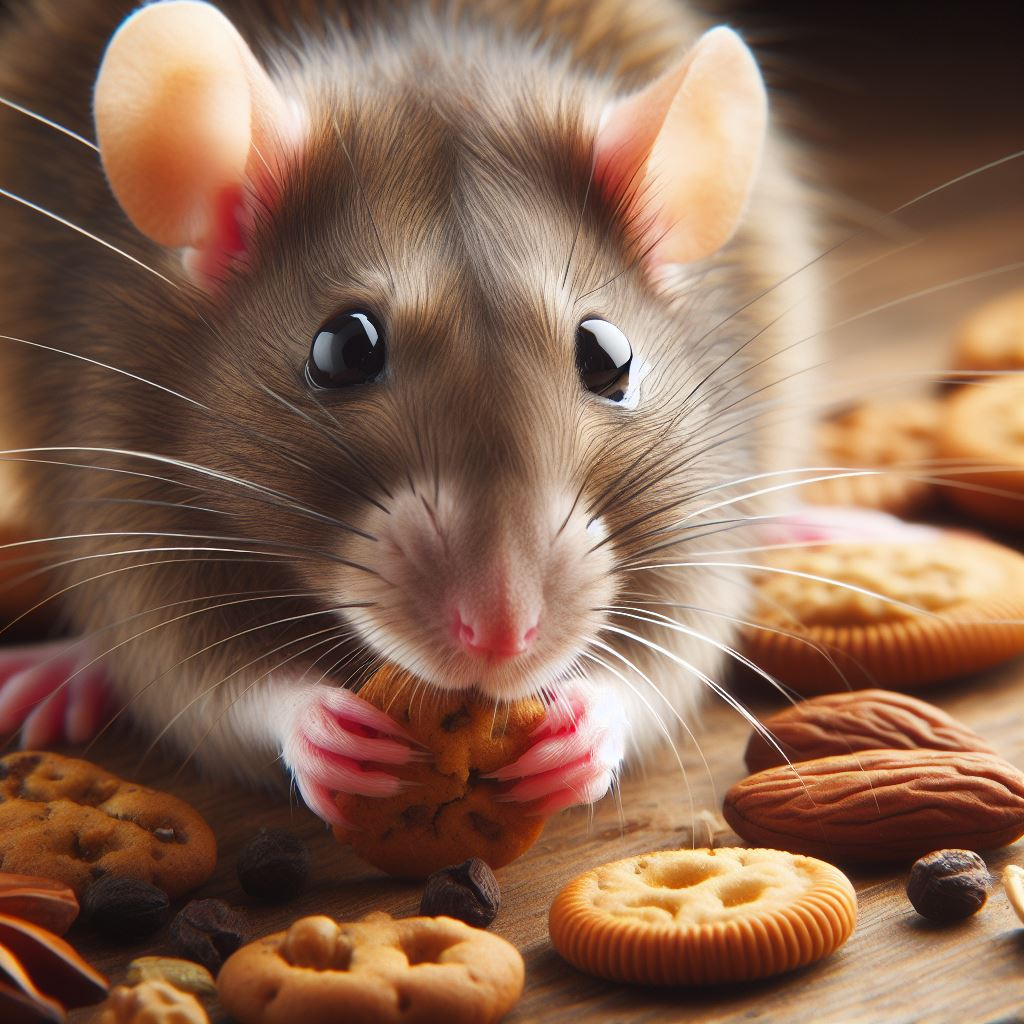
\includegraphics[width=0.4\textwidth]{rat.jpeg}
    \caption{Картинка сгенерирована нейросетью.}
\end{figure}
\newpage

\addsubsection{Задание №1}
Совместные функции распределения равняются произведению одномерных функций распределений каждой из переменных. Поэтому нам достаточно проверить выполнение свойств функции распределения случайной величины для каждой из переменных:
\begin{enumerate}
    \item $F(x, y) \to 0$ при $x, y \to -\infty$, $F(x, y) \to 1$ при $x, y \to \infty$
    \item $F(x, y)$ монотонно возрастает
    \item $F(x, y)$ непрерывна справа
\end{enumerate}
\addsubsection{Задание №3}
Предположим, что $Y$ --- распределение Коши. Тогда плотность вероятности можно будет выразить через плотность вероятности $X$:
$$f_Y(x) = \frac{1}{|a|}f_X\left( \frac{x - b}{a} \right) = \frac{1}{|a|\pi\gamma \left( 1 + \left( \frac{x - b - x_0}{a\gamma} \right)^2 \right)}$$
\addsubsection{Задание №4}
$$\int_{-\infty}^{\infty}\int_{-\infty}^{\infty}p(x, y)dxdy = 1 \quad\Rightarrow\quad \int_{0}^{1}\int_{0}^{1}C(x^3+y^2-2xy)dxdy = \int_{0}^{1}\frac{Cx^4}{4}+Cxy^2-2C\frac{x^2}{2}y\at^1_0dy = \int_{0}^{1}\left( \frac{C}{4}+Cy^2-Cy \right)\at^1_0 =$$
$$= \frac{C}{4} + \frac{C}{3} - \frac{C}{2} = 1 \Rightarrow \frac{C}{12} = 1 \Rightarrow C = 12$$
\addsubsection{Задание №5}
Зная о том, что $X$ и $Y$ независимые, мы можем визуализировать $X + Y$ следующим образом: $X$ представляет собой количество успехов в первой серии испытаний, $Y$ --- количество успехов во второй серии испытаний. Когда мы суммируем $X$ и $Y$, мы фактически объединяем обе серии испытаний в одну большую серию испытаний. Таким образом, общее количество испытаний становится $n+m$, а вероятность успеха в каждом испытании остается той же --- $p$.
$$C^k_np^kq^{n-k}+C^k_mp^kq^{m-k} = p^k\left( C^k_nq^{n-k} + C^k_mq^{m-k} \right)$$
\addsubsection{Задания №7}
Например, пусть у вас есть случайная величина $X$, которая представляет собой количество времени за день, проведенного в смартфоне. Если у вас есть большой процент дней, когда вы не пользуетесь смартфоном вовсе, то медиана может быть равна нулю. Или, например, массив из пяти чисел: $[0, 0, 0, 1, 2]$ --- его медиана равна 0 и массив удовлетворяет условиям для неотрицательной случайной величины. 
\addsubsection{Задания №8}
Для зависимых (или по-другому говоря, коррелируемых) $X, Y$ дисперсия суммы выражается через ковариацию: $Var(X + Y) = Var(X) + Var(Y) + 2Cov(X, Y)$. Данное в задании равенство выполняется только для некореллированных величин, когда ковариация равна нулю. 
\addsubsection{Задания №9}
Можно привести и другой пример случайной величины с такой плотностью распределения:
$$R(x) = \begin{cases}
    0,&x \in(-\infty, 1)\\
    \frac{1}{x^2},&x \in (1, \infty)
\end{cases}$$
Вычислить мат.ожидания для такого распределния не получится, потому что перед нами будет расходящийся интеграл, который мы не сможем вычислить.
\end{document}